\subsection{Hello World Example}

\begin{minted}[breaklines]{c++}
int main {
    // This is a comment
    std::cout << "Hello World from C++!" << std::endl;
    std::cout << "I am using the default style to print this code in beautiful colors. Since the text is so long I have to include the 'breaklines' option as well" << std::endl;
    return 0;
}
 
\end{minted}

\vdots

\usemintedstyle{rrt}
\begin{minted}{python}
# This is a comment
print('Hello world from Python!')
print('I am using the "rrt" style to print this code in beautiful colors')
\end{minted}

\vdots

\usemintedstyle{tango}
\inputminted[breaklines]{Matlab}{./Code/HelloWorld.m}

\subsection{Flow Chart Example}

\begin{center}
\begin{tikzpicture}[node distance = 2cm, auto]
    % Place nodes
    \node [block] (init) {Learning \LaTeX};
    \node [cloud, left of=init] (you) {You};
    \node [block, below of=init] (new_project) {Making new project};
    \node [decision, below of=new_project] (decide) {Is the template good enough?};
    \node [block, right of=new_project, node distance=3cm] (no) {Improve the template};
    \node [block, below of=decide, node distance=3cm] (yes) {Get to work!};

    % Draw edges
    \path [line] (init) -- (new_project);
    \path [line] (new_project) -- (decide);
    \path [line] (decide) -- node {Yes} (yes);
    \path [line] (decide) -| node [near start] {No} (no);
    \path [line] (no) -- (new_project);
    \path [line,dashed] (you) -- (init);
\end{tikzpicture}
\end{center}

\subsection{Sub-figures Example}
\begin{figure}[H]
    \centering
    \begin{subfigure}[t]{0.450\textwidth}
        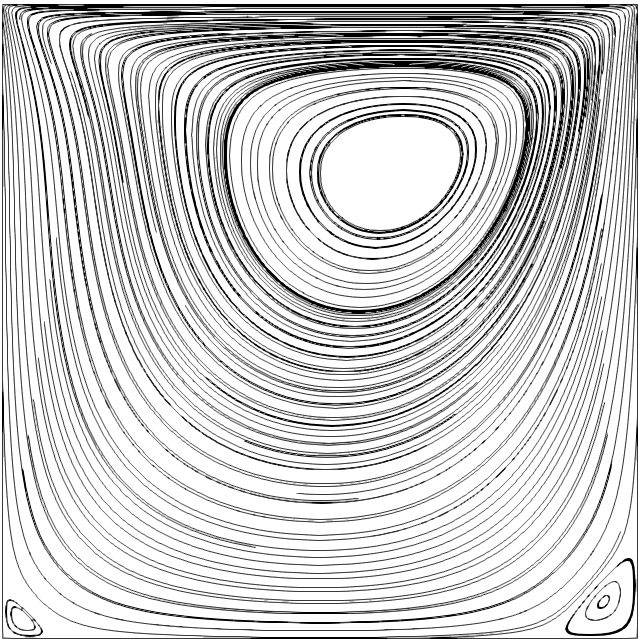
\includegraphics[width=\textwidth]{Images/Sub-figures_Example/cavity_100_streamlines.png}
        \caption*{$Re = 100$ - Exercise}
    \end{subfigure}
    \begin{subfigure}[t]{0.441\textwidth}
        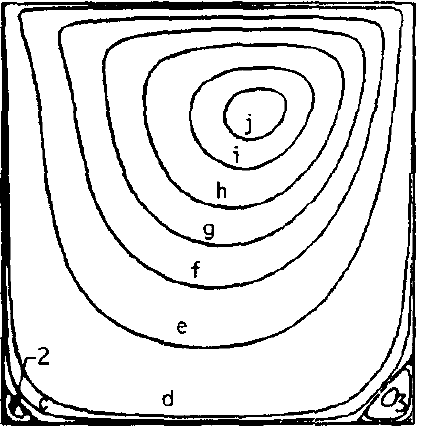
\includegraphics[width=\textwidth]{Images/Sub-figures_Example/cavity_100_streamlines_ghia.png}
        \caption*{$Re = 100$ \parencite{ghia_1982}}
    \end{subfigure}
    \\  % This makes a new line
    \begin{subfigure}[t]{0.450\textwidth}
        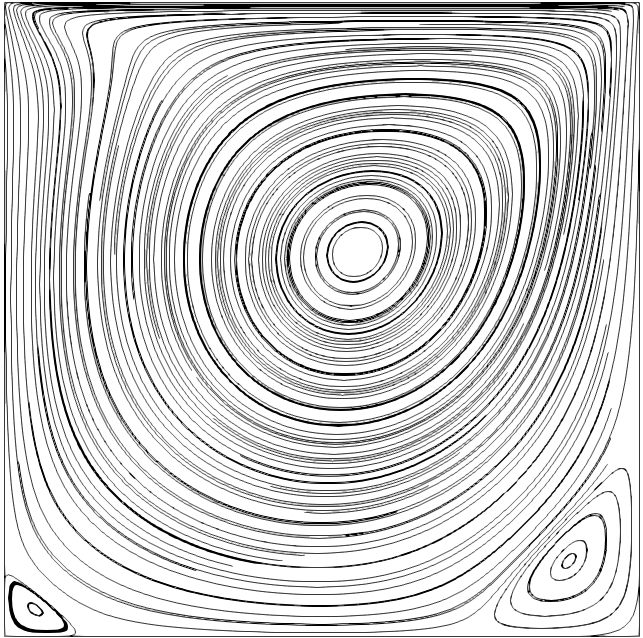
\includegraphics[width=\textwidth]{Images/Sub-figures_Example/cavity_400_streamlines.png}
        \caption*{$Re = 400$ - Exercise}
    \end{subfigure}
    \begin{subfigure}[t]{0.438\textwidth}
        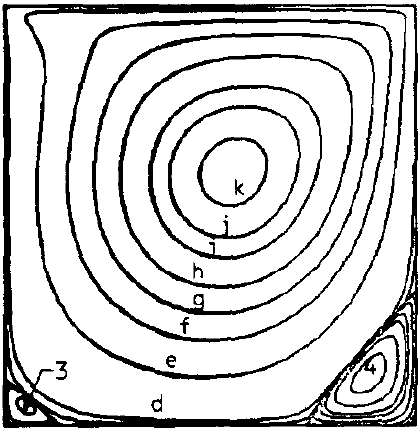
\includegraphics[width=\textwidth]{Images/Sub-figures_Example/cavity_400_streamlines_ghia.png}
        \caption*{$Re = 400$ \parencite{ghia_1982}}
    \end{subfigure}
    \\  % This makes a new line
    \begin{subfigure}[t]{0.450\textwidth}
        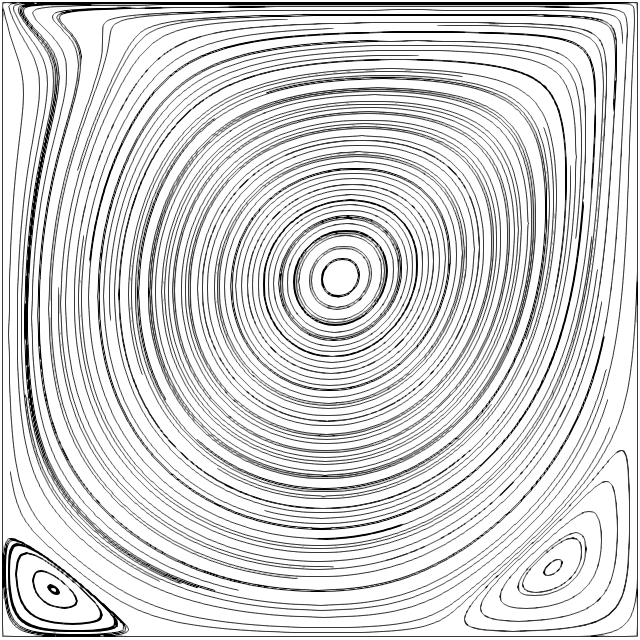
\includegraphics[width=\textwidth]{Images/Sub-figures_Example/cavity_1000_streamlines.png}
        \caption*{$Re = 1000$ - Exercise}
    \end{subfigure}
    \begin{subfigure}[t]{0.438\textwidth}
        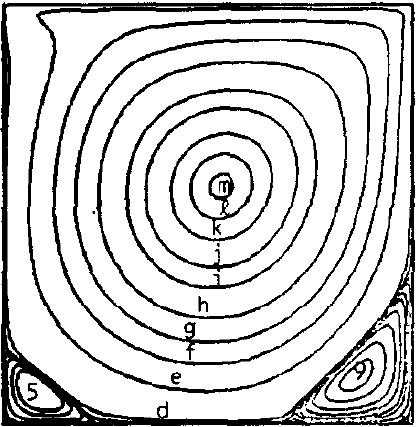
\includegraphics[width=\textwidth]{Images/Sub-figures_Example/cavity_1000_streamlines_ghia.png}
        \caption*{$Re = 1000$ \parencite{ghia_1982}}
    \end{subfigure}
    \caption[Streamline results]{Streamlines for the problem of a lid-driven cavity.}
    \label{fig:cavity_streamline}
\end{figure}